\documentclass[aps,pre,twocolumn,letterpaper,floatfix,showpacs]{revtex4}
\usepackage{graphicx} 
\usepackage{amsmath,amssymb,amsfonts} 
\usepackage{mathtools}
\usepackage{pdfpages}
\usepackage{afterpage}
\usepackage[hidelinks]{hyperref} 
\usepackage{epstopdf}
\usepackage{color}
\definecolor{Blue}{rgb}{0.1,0.1,1.0} 
\definecolor{Magenta}{rgb}{1.0,0.1,0.5} 
\definecolor{LRed}{rgb}{0.8,0.0,0.0} 

 \newcommand{\todo}[1]{ {\color{Magenta} TODO: \color{Blue} \textbf{#1} }}


\begin{document}
\title{Structural replication of nanoporous media using procedural noise}
%\author{A. Hafreager, N. Groeneboom, A. Malthe-S\oe renssen$^1$}
\email{anders.hafreager@fys.uio.no}
\author{Anders Hafreager $^{1}$} 
\author{Nicolaas Groeneboom $^{1}$} 
\author{Anders Malthe-S\o renssen $^1$}
\affiliation{$^1$Department of Physics - University of Oslo\\Sem S{\ae}lands vei 24, NO-0316, Oslo, Norway }
\date{\today} 

%%%%%%%%%%%%%%%%%%%%%%%%%%%%%%%%%%%%%%%%%%%%%%%%%%%%%%%%%%%%%%
%%%%%%%%%%%%%%%%%%%%%%%%%%%%%%%%%%%%%%%%%%%%%%%%%%%%%%%%%%%%%%
\begin{abstract} 
In this paper, we aim to develop a method for producing statistically correct simulations of nanoporous media without the use of conventional Molecular Dynamics Simulator (MDS). In short, the proposed model is a binary function that returns either true if the input position is in a void / pore, or false if within a wall. By using procedural noise, we are not restricted to generating media within a limited box, as the noise functions is continuous on all scales. It is therefore possible to validated pores at theoretically arbitrary range. In addition, this method is extremely fast, requiring very little computational power to calculate whether a particle is within a pore or not. After presenting such a model, we choose a method to measure the structural properties of nanoporous media that are created either through regular methods (e.g. LAMMPS) or with our method. The measure we selected is the radial pore size distribution $g(r)$, which is regarded as the de-facto standard method for capturing the structural properties of porous media. Using this measure, we define a full likelihood framework for estimating model parameters given any data set, and continue by validating our own framework by analysing procedural noise data sets with known input parameters. Finally, we perform a full likelihood analysis of silica $SiO^2$ data set simulated in LAMMPS, and show that our model correctly reproduces several of the internal properties of the data set, including $g(r)$, porosity and surface area.     

\end{abstract} 
 
\maketitle
 
% %%%%%%%%%%%%%%%%%%%%%%%%%%%%%%%%%%%%%%%%%%%%%%%%%%%%%%%%%%%%%
%% %%%%%%%%%%%%%%%%%%%%%%%%%%%%%%%%%%%%%%%%%%%%%%%%%%%%%%%%%%%%
\section{Introduction}


Lorem ipsum dolor sit amet, consectetur adipiscing elit. Duis consequat turpis vel mollis accumsan. Etiam eleifend magna vel quam porta, sed porta nibh placerat. Sed in faucibus risus. Duis suscipit tincidunt leo, nec laoreet leo elementum elementum. Pellentesque habitant morbi tristique senectus et netus et malesuada fames ac turpis egestas. Sed eros risus, convallis sit amet turpis a, dapibus accumsan quam. Donec fringilla rhoncus turpis, quis ultrices odio vulputate elementum. Cras nec viverra urna. Phasellus laoreet tortor sed est sagittis laoreet. Nullam a volutpat ex.

Mauris vestibulum sit amet libero eget facilisis. Vivamus a nunc sed felis ultrices convallis luctus et mauris. Sed tincidunt mauris nunc, vehicula placerat eros faucibus quis. Morbi egestas, nisi quis luctus dignissim, mauris odio pulvinar tellus, non efficitur risus erat vel nunc. Cras vel felis magna. Mauris rutrum magna a interdum sodales. Nam tempor, diam non sodales tristique, nulla ipsum eleifend dui, non aliquam felis tellus id enim. Donec eget nulla leo.

Ut hendrerit cursus libero, in scelerisque tortor sollicitudin accumsan. Nam eleifend velit metus, quis volutpat justo faucibus ut. Cras ut sem in nunc fringilla egestas vitae sit amet justo. Ut vel condimentum tortor. Morbi in massa in ipsum ultrices tincidunt. Duis feugiat dignissim nisi ac ultricies. Quisque eget risus fermentum, condimentum massa ullamcorper, posuere neque. Nam congue consequat mi, vel commodo mi tempus eget.

Nullam ultrices, velit sed venenatis ultrices, risus urna ultricies magna, at pretium lorem nibh et nunc. Suspendisse sed mattis leo. Nulla facilisi. Praesent finibus lobortis leo, ut porttitor massa tincidunt ut. Vivamus quis orci eu sem sodales ornare. Cras sed faucibus velit. Phasellus scelerisque mauris quis lorem dignissim vehicula. Sed tempor ut urna sed bibendum. Donec et nibh pulvinar, commodo magna ac, interdum nibh. Sed laoreet ipsum quis quam lacinia, in dictum erat laoreet. Etiam rhoncus mauris arcu, ac egestas lacus facilisis nec. Pellentesque a orci vitae felis faucibus ultrices sed non massa. In posuere vel ex in elementum. Aenean ac neque a enim gravida tristique eu ac lacus. Ut tincidunt venenatis lectus, et maximus mauris.

Proin ornare nulla id tristique placerat. Integer nec elementum tellus. Cras at tempus lectus. Cras lorem est, ornare id condimentum vitae, scelerisque eu lectus. Aenean libero arcu, consequat vel sagittis eget, sagittis ut neque. Pellentesque habitant morbi tristique senectus et netus et malesuada fames ac turpis egestas. Aenean nec quam sodales, mollis est sit amet, vulputate turpis. Praesent tempus diam eu sem laoreet finibus. Nulla finibus, sapien vel lobortis ultricies, mauris ipsum aliquet urna, quis rutrum sapien dui id ipsum. Quisque sodales ex sapien, ac egestas lacus suscipit et. Suspendisse accumsan rhoncus tristique. Pellentesque ut eros lectus. Praesent viverra sit amet odio nec vulputate. Class aptent taciti sociosqu ad litora torquent per conubia nostra, per inceptos himenaeos. Nulla molestie metus vitae libero vulputate, at interdum enim tempus.

\section{Method}
\todo{her står det nå det samme som i abstract}
In this paper, we aim to develop a method for producing statistically correct simulations of nanoporous media without the use of conventional Molecular Dynamics Simulator (MDS). In short, the proposed model is a binary function that returns either true if the input position is in a void / pore, or false if within a wall. By using procedural noise, we are not restricted to generating media within a limited box, as the noise functions is continuous on all scales. It is therefore possible to validated pores at theoretically infinite range. In addition, this method is extremely fast, requiring very little computational power to calculate whether a particle is within a pore or not. 

After presenting such a model, we choose a method to measure the structural properties of nanoporous media that are created either through regular methods (e.g. LAMMPS \cite{plimpton1995fast}) or with our method. The measure we selected is the radial pore size distribution $g(r)$, which is regarded as the de-facto standard method for capturing the structural properties of porous media. 

Using this measure, we define a full likelihood framework for estimating model parameters given any data set, and continue by validating our own framework by analysing procedural noise data sets with known input parameters. Finally, we perform a full likelihood analysis of  

\subsection{Procedural noise}
\label{sec:perlin}

Procedural algorithmic methods for creating realistic-looking
fractal-like patterns have been around for more than 30 years. The most famous of these
algorithms is Perlin noise, first developed by Ken Perlin in 1982 for
use in the movie ``Tron''.  Perlin noise is a type of pseudo-random
gradient noise that mimics a Gaussian field, but at low computational cost. 
An improved version of Perlin noise is called Simplex
noise, which has several advantages over standard Perlin noise in
terms of scalability and speed.  


\subsubsection{Perlin noise - an overview}
An overview of the current state of procedural noise functions can be
found in \cite{lagae:2010}.  Perlin noise \citep{perlin:2002} 
is a band limited repeatable pseudo-random function
from $\mathbb R^n \to \mathbb R$ that is computationally fast and has
properties which make it suitable for creating patterns that mimic
nature. Perlin noise is an approximation to Gaussian filtered noise
implemented as a pseudo-random spline. The algorithm uses a predefined
grid of gradients pointing in a random direction, where for any point
within a grid, we interpolate the gradients from the four corners. The
algorithm is as follows:
\begin{itemize}
  \item[1.] For a point, obtain the four closest gradients in the grid.
   \item [2.] For each of the gradients, calculate the dot product
     between the gradient and a vector defined by the  the distance
     between the the point and the current grid corner. 
   \item [3.] Instead of linear interpolation $F(t) = t$, use a fade function to produce smoother interpolated values. Perlin noise typically uses the following fade function: $F(t) = t ^3 (t  (6 - 15) + 10)$.
    \item [4.] Obtain the final value by linearly interpolating between the x-axis and
      use this result to linearly interpolate the y-axis. 
\end{itemize} 
Simplex noise works in a similar manner, but requires fewer
computational steps, scales better in higher ($\ge 3$) dimensions and has fewer 
anisotropic properties. 

\subsubsection{Properties of procedural noise}
\begin{figure}
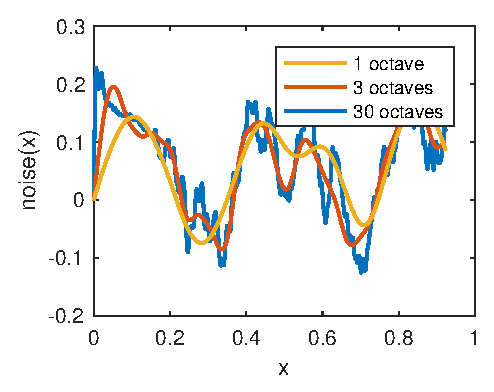
\includegraphics[width=.5\textwidth]{noise.eps}
\caption{Perlin noise (left) versus simplex noise (right). Note the
  straight x-y pattern in the single upper Perlin mode and the less
  anisotropic simplex mode. Lower part: combining octaves tend
  to remove these patterns.}
\label{fig:noise}
\end{figure}

\begin{figure}
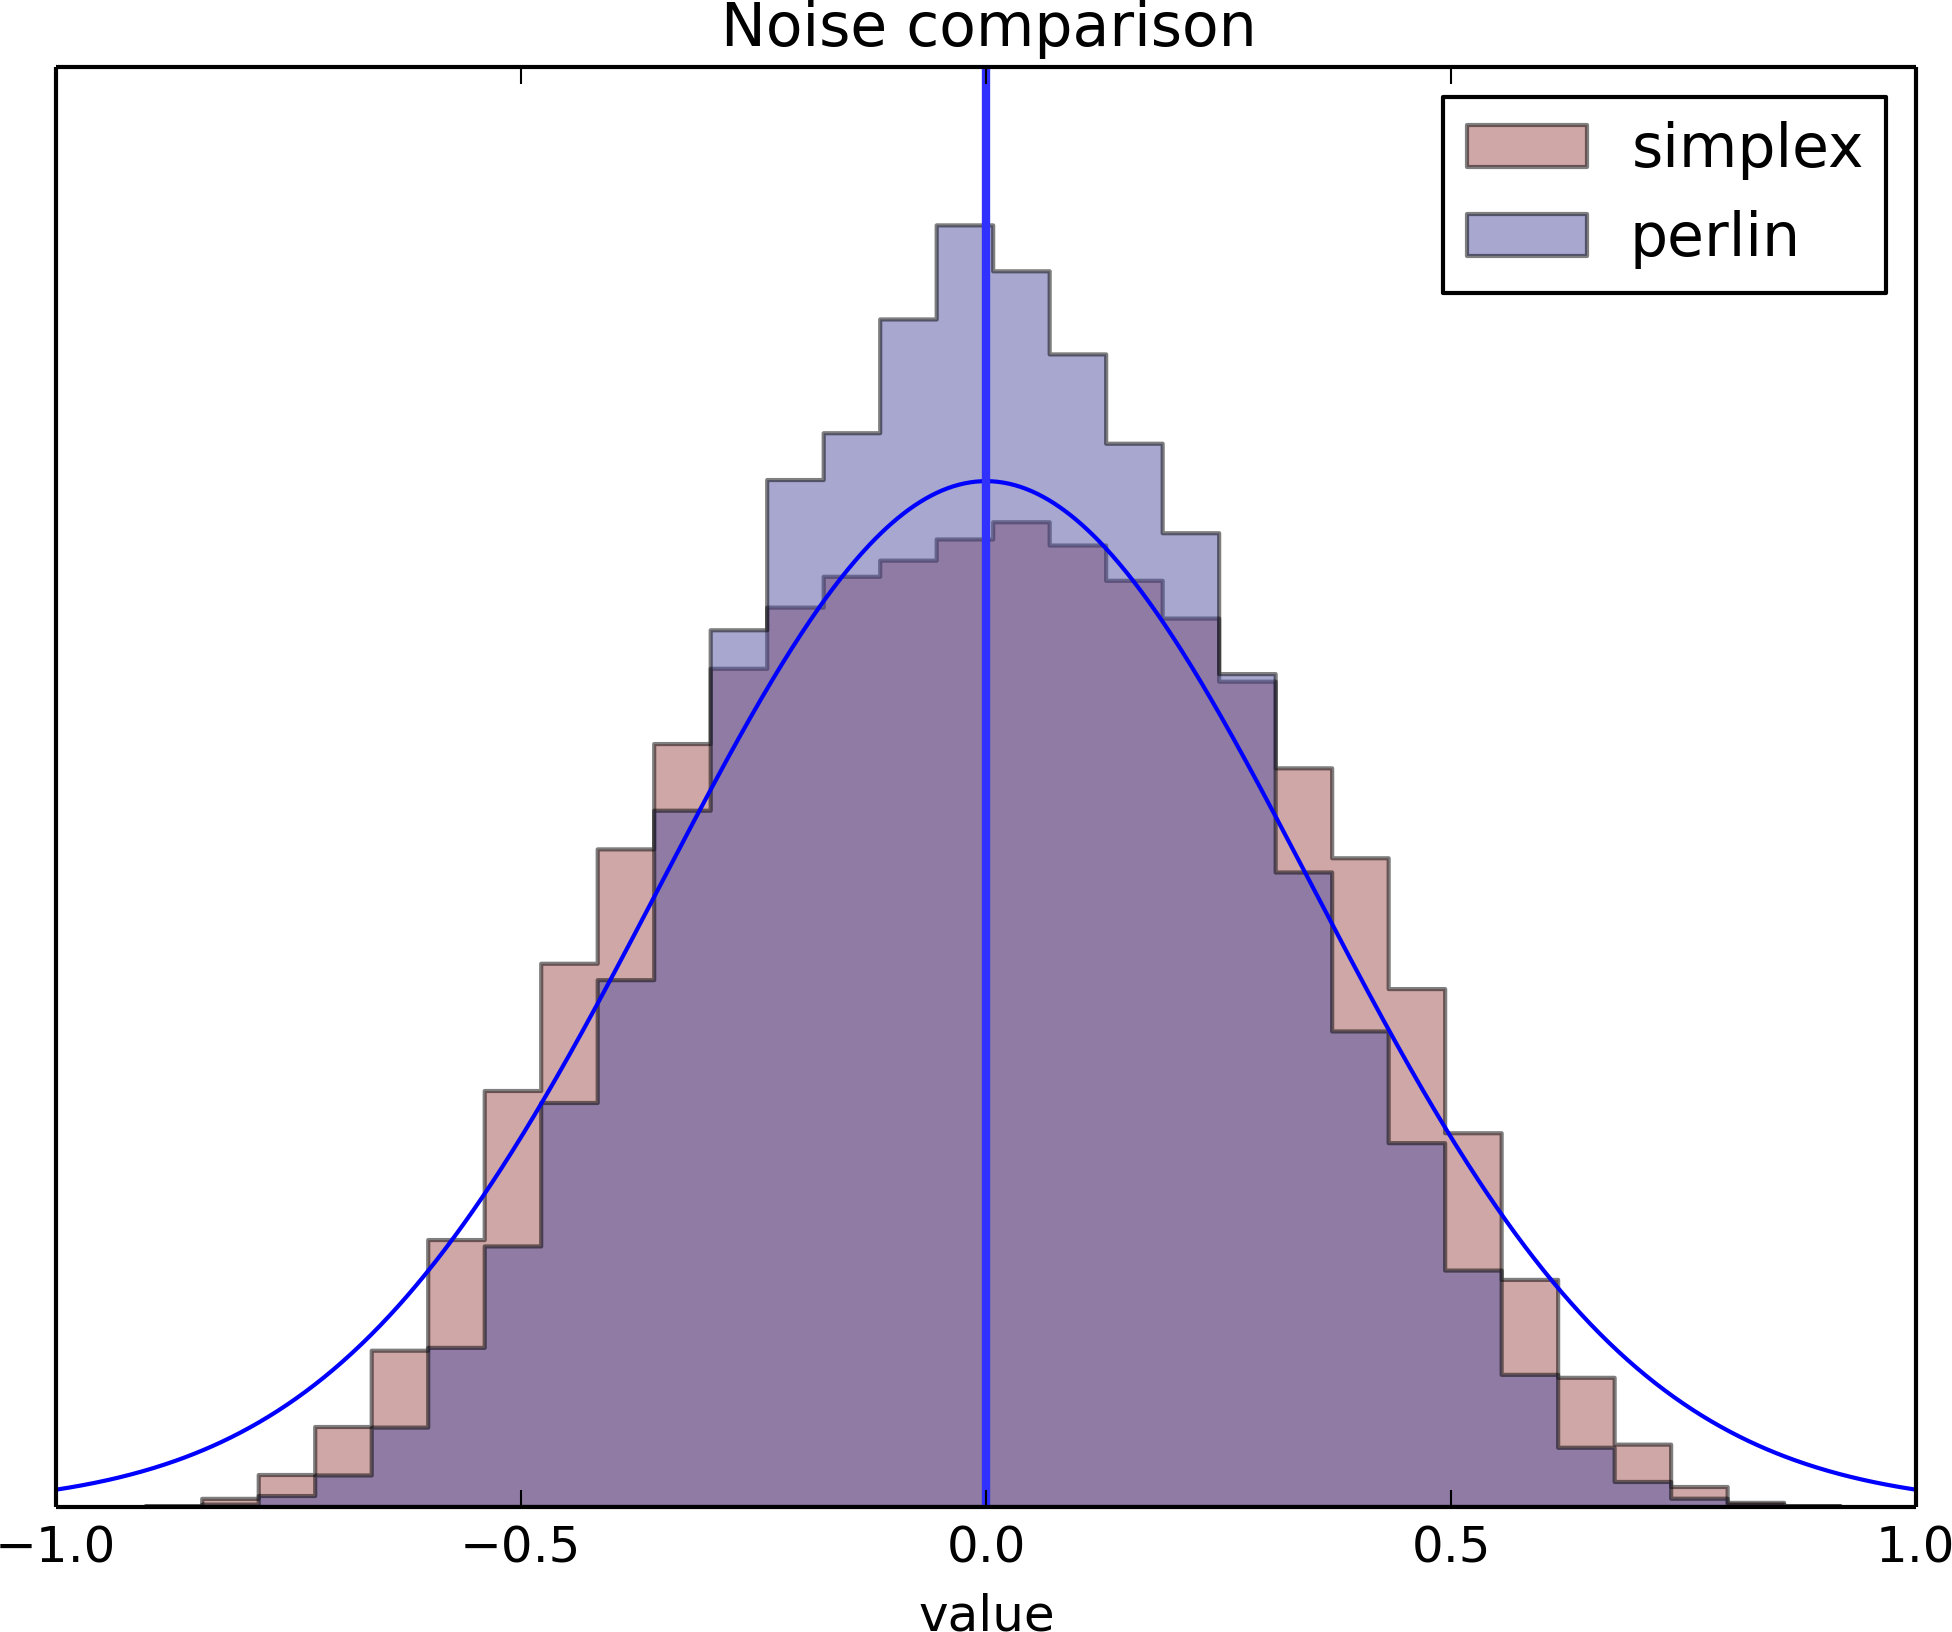
\includegraphics[width=.5\textwidth]{noise_comparison.png}
%\mbox{\epsfig{file=perlinstats.eps, width=\linewidth}}
\caption{Normalized distributions of Perlin noise and simplex noise compared with a
  Gaussian distribution. Note how both noise functions produce
  near-Gaussian, but slightly different distributions.}
\label{fig:properties}
\end{figure}
Standard Perlin noise is known for having several anisotropic features
\citep{lagae:2010}. Perlin noise also gives rise to a ``textile''
pattern in the $x$ and $y$-directions, which is evident from the upper
left part of figure \ref{fig:noise}, depicting 2D Perlin noise in
a single octave. The upper-right part shows the same node for Simplex noise,
with less obvious patterns. However, when combining several octaves,
as depicted in the two lower parts, these anisotropic patterns tend to cancel
out. In any case, for observations of weak gravitational lensing, these anisotropies would occur on much smaller 
scales than the typical resolution. 
In addition, we have calculated the statistical distributions for Perlin and simplex noise
with $\sigma = 0.3$, and have plotted the results in figure \ref{fig:properties}.
Each procedural noise method has distributions that are close to normal, 
but with some asymmetrical properties. 



\subsection{Multiple octaves: creating patterns}
\label{sec:octaves}
The different octaves from procedural noise functions can be combined
to produce a wide range of nature-like patterns. A generic
N-dimensional procedural function $\Phi(\vec x): \mathbb R^N \to
\mathbb R$ could be expressed as
\begin{equation}
\label{eq:procedural}
 \Phi(\vec x) = \Theta \Big(\sum_k \kappa (k) P(  f_s (\vec x,k) )) \Big),
 \end{equation}
where $f_s(\vec x,k)$ describes the frequency scale modifier (e.g. $f_s(\vec x,k) =
k\vec x$), $\kappa(k)$ is the octave amplitude (eg $\kappa(k) = 1/k$)
and $\Theta(x)$ an overall modifier (e.g. $\Theta(x) = x$ or
$\Theta(x) = \frac{1}{x}$). In a sense, $\kappa(k)$ is similar to Fourier coefficients. 
In its simplest case, summing directly
over the octaves with amplitude $1/k$ results in 
\begin{equation}
\label{eq:perlinlinear}
 \Phi(\vec x) = \sum_k \frac{1}{k} P( 2k\vec x), 
\end{equation}
and produces an 2D procedural noise pattern depicted in the lower
part of figure \ref{fig:noise}. Finally, since simplex noise both scales better with higher dimensions and produces less asymmetric effects, we choose to use this noise method over regular Perlin noise in our method.  

\subsection{Model}
In this paper, we are interested in developing a model using Simplex/Perlin noise to reproduce nanoporous structures that are as statistically close to actual simulations of porous media. For a given data set and a model, we wish to estimate the parameters that best represent the data. This is performed through a full likelihood analysis, where we in addition validate the model by comparing the radial pore size distribution $g(r)$, porosity and surface area of the system.  

\begin{figure*}
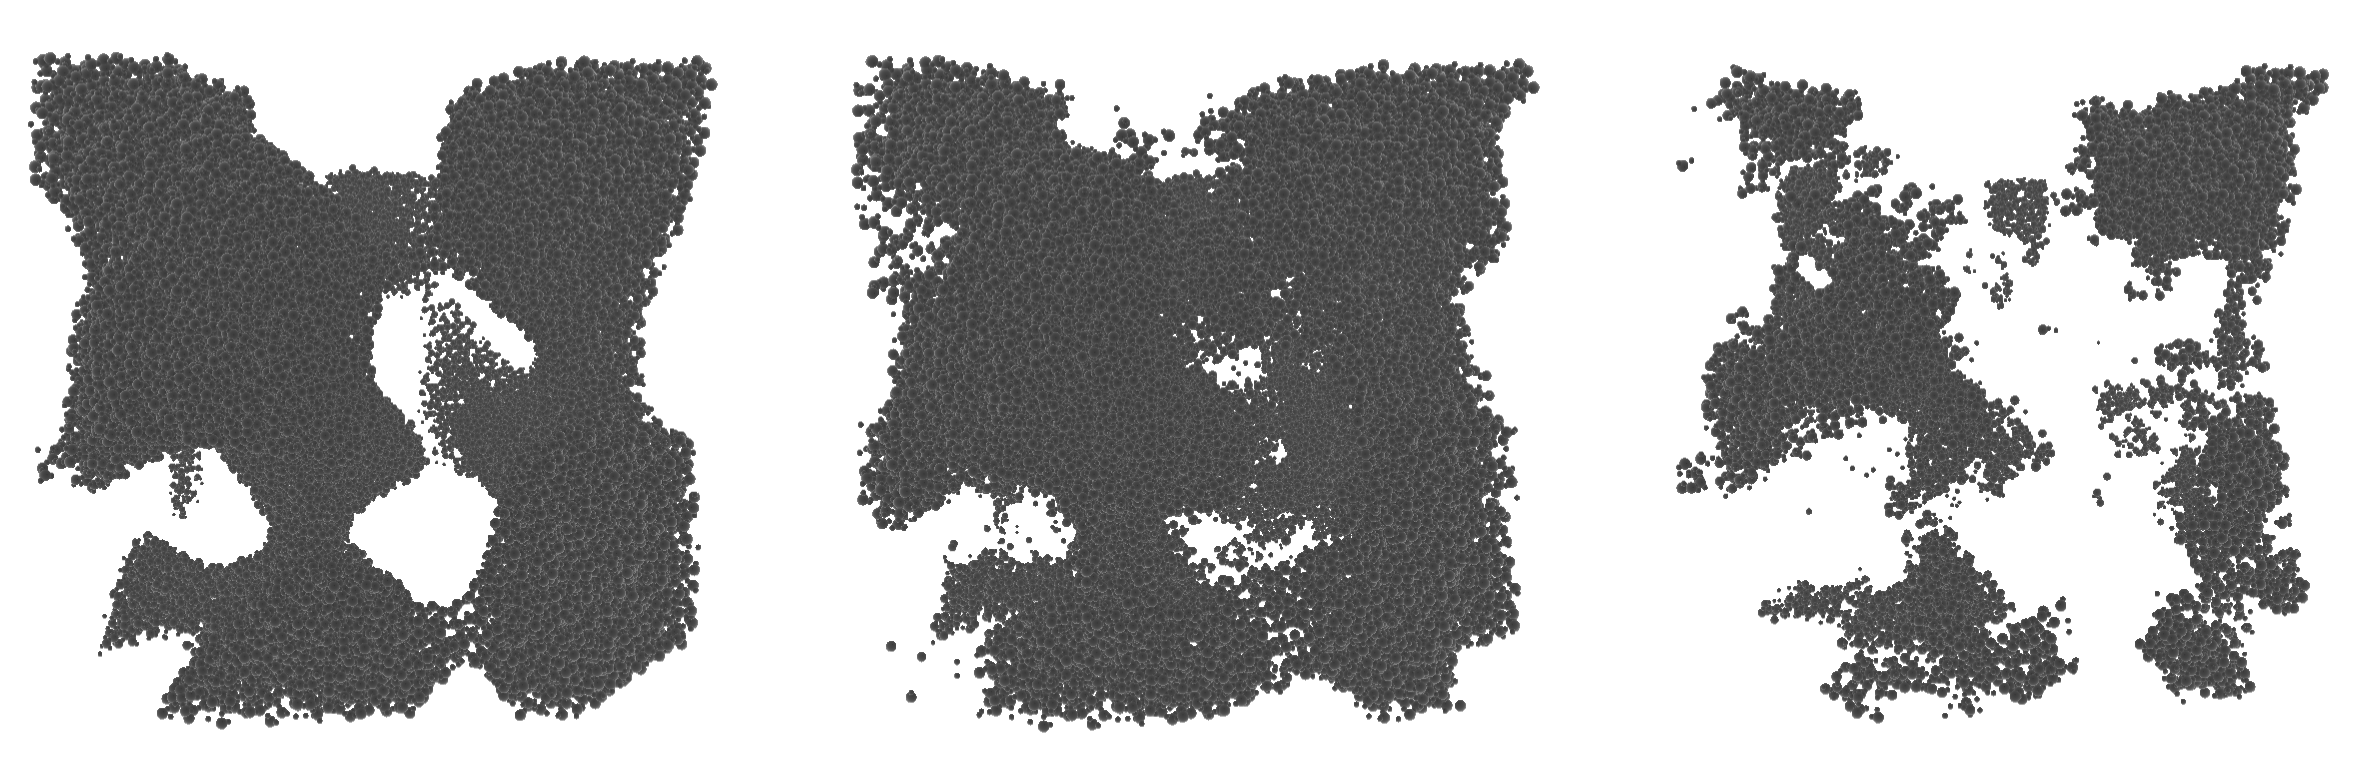
\includegraphics[width=.95\textwidth]{model_examples.png}
\caption{Examples of 3D simplex noise structures in nanoporous media. Left image: low persistence (large scale dominates), middle image: medium persistence (small scales starts dominating) and right image: high threshold (more atoms are discarded). }
\label{fig:model_example}
\end{figure*}
We construct a generic sum over procedural noise octaves with the expression: 
\begin{equation}
  M_1(\vec x) = \sum_{\omega=0}^{\Omega} \psi^{\omega -1}   N\big((\vec x + \sigma \cdot \omega)\nu \cdot 2^{\omega-1} \big),
\label{eq:noisemodel1}
\end{equation}
where $\Omega$ is the total amount of octaves, $\psi$ the persistence (scale falloff), $N$ a generic $N$-dimensional noise function, $\sigma$ a predefined random vector that removes anisotropic artefacts and $\nu$ the frequency modifier representing the initial largest scales in the model. For each mode, the frequency is thus multiplied, while the overall amplitude is damped by a given persistence. In the end, we simulate a large set of bulk particles without any walls, and use the noise function to remove particles that are not in a procedural void given by a threshold $\tau$. Three examples of this model are depicted in figure \ref{fig:model_example}, where we have used $\Omega=6$ octaves and the scale is $\nu=0.01$ and cut-off $\tau=0$. The left image depicts low persistence ($\psi = 0.0$), where only the first octave dominates (corresponding to large scales). The middle picture shows the same parameters with a higher persistence $(\psi = 0.5)$, where smaller scales become more dominating. In the rightmost picture, the effect of the cut-off threshold $\tau = -0.3$ is shown.   


\subsection{Model Measure}
In order to perform data analysis on the model parameters, we developed a code that uses Monte Carlo Markov chains in order to produce samples for building the likelihood. Before doing so, we need a model measure - a quantitative method that characterizes the internal structure of the porous media. This quantity should be computed for both the original data set and the one produced by our noise model. 

Ideally, the model measure should pick up all geometrical properties that are relevant for the physical study of interest. For instance, pore size distribution and porosity are import for studying transport in porous media. Another such measure is the Distance-To-Atom (DTA).
The method used for calculating the porosity of a media is defined as in \cite{gelb1998characterization}, and we obtain the surface area of a porous media by using marching cubes triangulation to sum the surface area of the triangles. 

In this paper, we choose to use the radial pore size distribution $g(r)$ as defined and implemented in LAMMPS \cite{plimpton1995fast}.  \todo{skriv litt mer om hvorfor vi velger g(r)}





%\begin{figure}[htb!]
%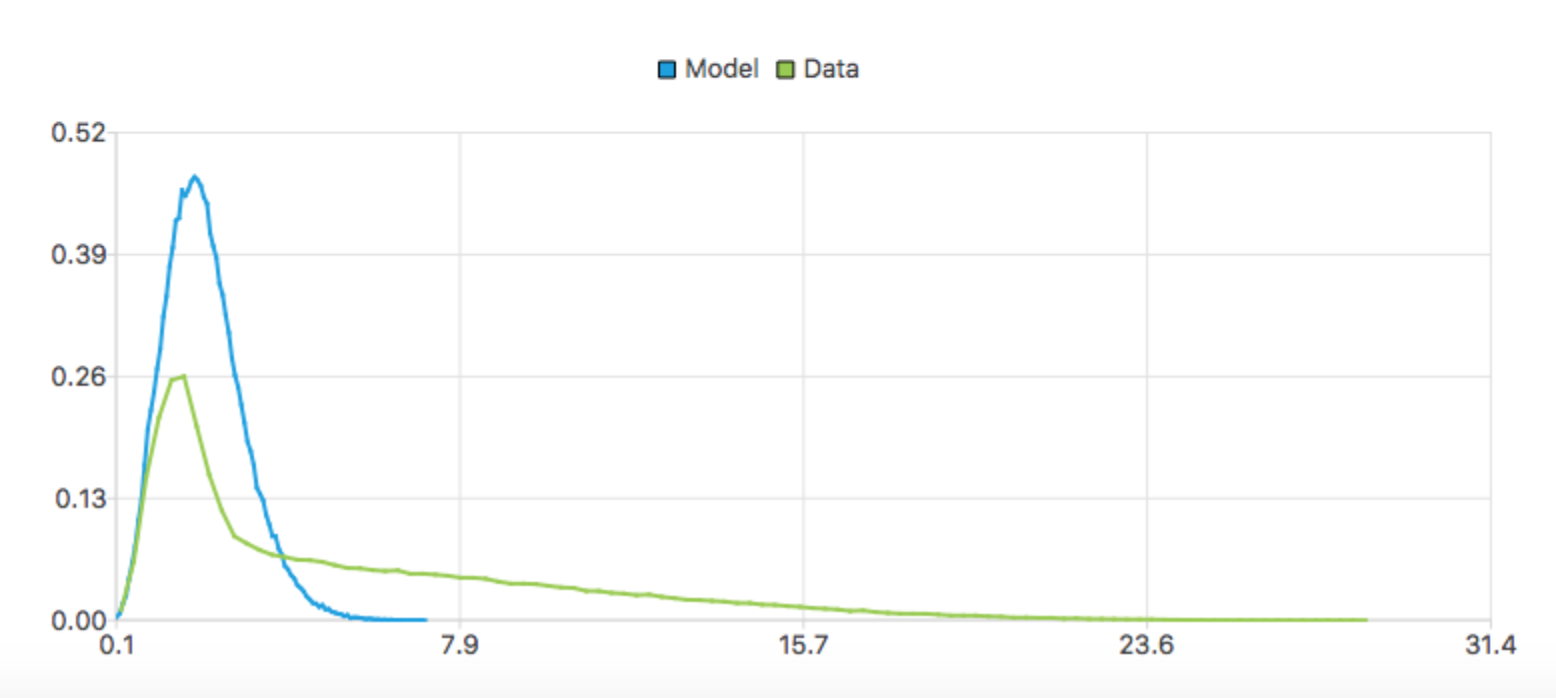
\includegraphics[width=.45\textwidth]{DTA.png}
%\caption{Distance-to-atom measure for two data sets with varying persistence. The green line corresponds to a mock data set with low persistence (dominated by large-scale modes), while the blue line corresponds to high persistence (dominated by small scale modes). }
%\label{fig:dta_example}
%\end{figure}



%\subsubsection{Fractal Dimension}
%The fractal dimension is a ratio providing a statistical index of complexity comparing how detail in a pattern changes with the scale at which it is measured. We provide a fracal

%\subsubsection{Octree Counting Measure (OCM)}

%\subsection{Diffusion Measure}

\subsection{Likelihood}
The likelihood $\mathcal{L}$ of parameters $\theta$ of a model $M(\theta)$ given outcome $x$ is defined as $\mathcal{L} (M(\theta) | x) = P( x | M(\theta))$, where P is the probability distribution. In our model, we use the $\chi^2$ test to fit our one-dimensional measure from the data $\bf d$ with our model $\bf M(\theta)$. Pearson's $\chi^2$ is defined as 
\begin{equation}
  \chi^2 = \sum_i \frac{ \Big(d_i - M(\theta)_i \Big)^2}{M(\theta)_i^2},
\end{equation}    
and the likelihood is thus
\begin{equation}
\mathcal L \propto e^{-\chi^2}.
\end{equation}
For a model with $N$ free parameters, we build the full $N$-dimensional likelihood by letting random walkers map out the parameter space through the Monte Carlo Markov chain method (MCMC). For each step $M(\theta)_n$ in parameter space, we calculate the likelihood for this parameter configuration. Then, we create a new set of parameters for the next step $M(\theta)_{n+1}$ by choosing new parameters randomly from a $N$-dimensional sphere around the previous parameters. The model also chooses a new random seed. We calculate the likelihood at the new step and perform the MCMC test: Accept the new step if $\frac{\mathcal L_n}{\mathcal L_n+1} \ge 1$, or reject if the value is lower than a uniform random value $\in [0,1]$.  

\section{Model verification and data analysis}
\begin{figure}[htb!]
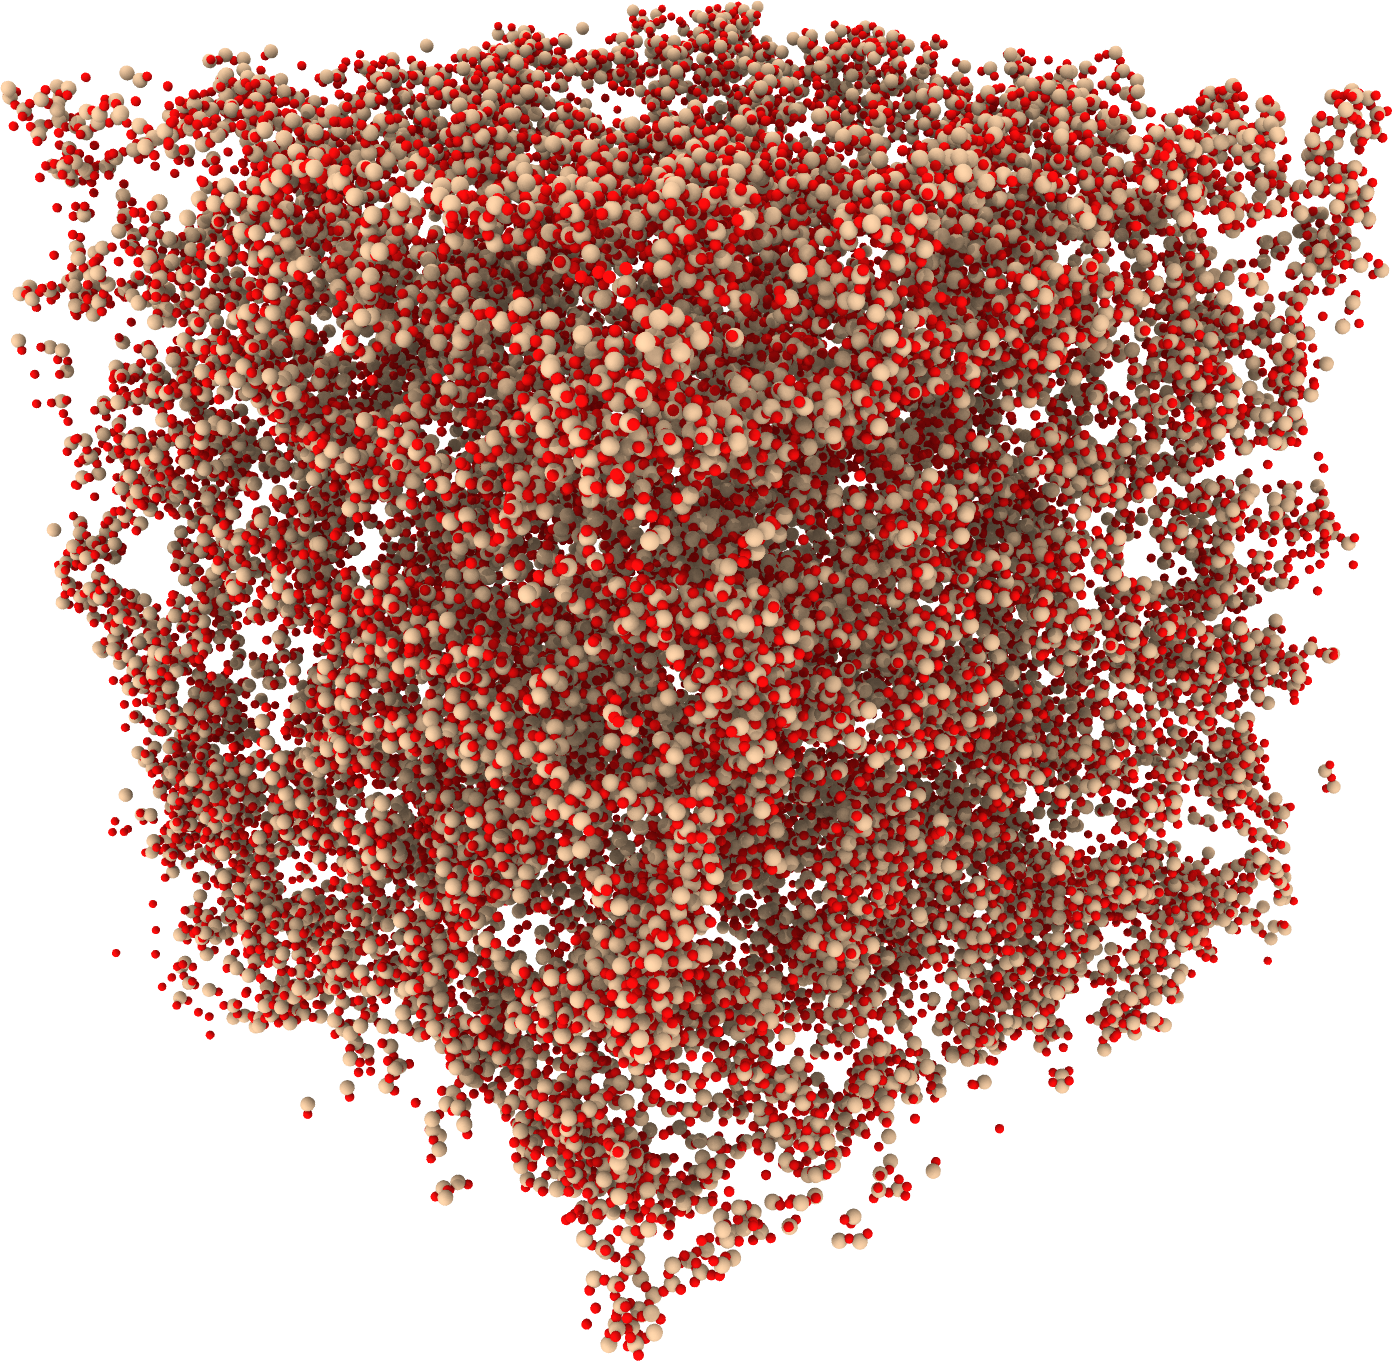
\includegraphics[width=.45\textwidth]{model_test.png}
\caption{Simulated mock data used for the initial model testing analysis. Input parameters are $\nu=0.03$,$\tau=-0.02$ and $\psi=0.6$.}
\label{fig:mockdata}
\end{figure}
In order to verify our likelihood code, we perform a model verification test on a mock data set with known input values. In this example, we only use standard simplex noise with three free parameters: the persistence $\psi$, threshold $\tau$ and scale $\nu$. We simulate a data set of $159 ^3 Å$ of $1 000 000$ atoms, and perform the cut-off given input parameters $\Omega=3$, $\Psi = 0.6$, $\tau=-0.2$, $\nu=0.03$. The resulting 3D structure is depicted in figure \ref{fig:mockdata}. 

We continue by performing a full MCMC analysis of the mock data with using a parallelized code running on a 48 core cluster. In order to produce 300 000 samples, about 48 hours was needed. The results from this analysis can be seen in figure \ref{fig:mockdataresults_pts}, where the upper panel depicts the marginalised 1D posteriors while the lower shows the marginalised 2D posteriors. The centre and left image shows that the input parameters of $\tau=-0.2$(threshold), $\psi=0.6$(persistence) and $\nu=0.03$ are all reproduced well within $1 \sigma$.


\begin{figure*}
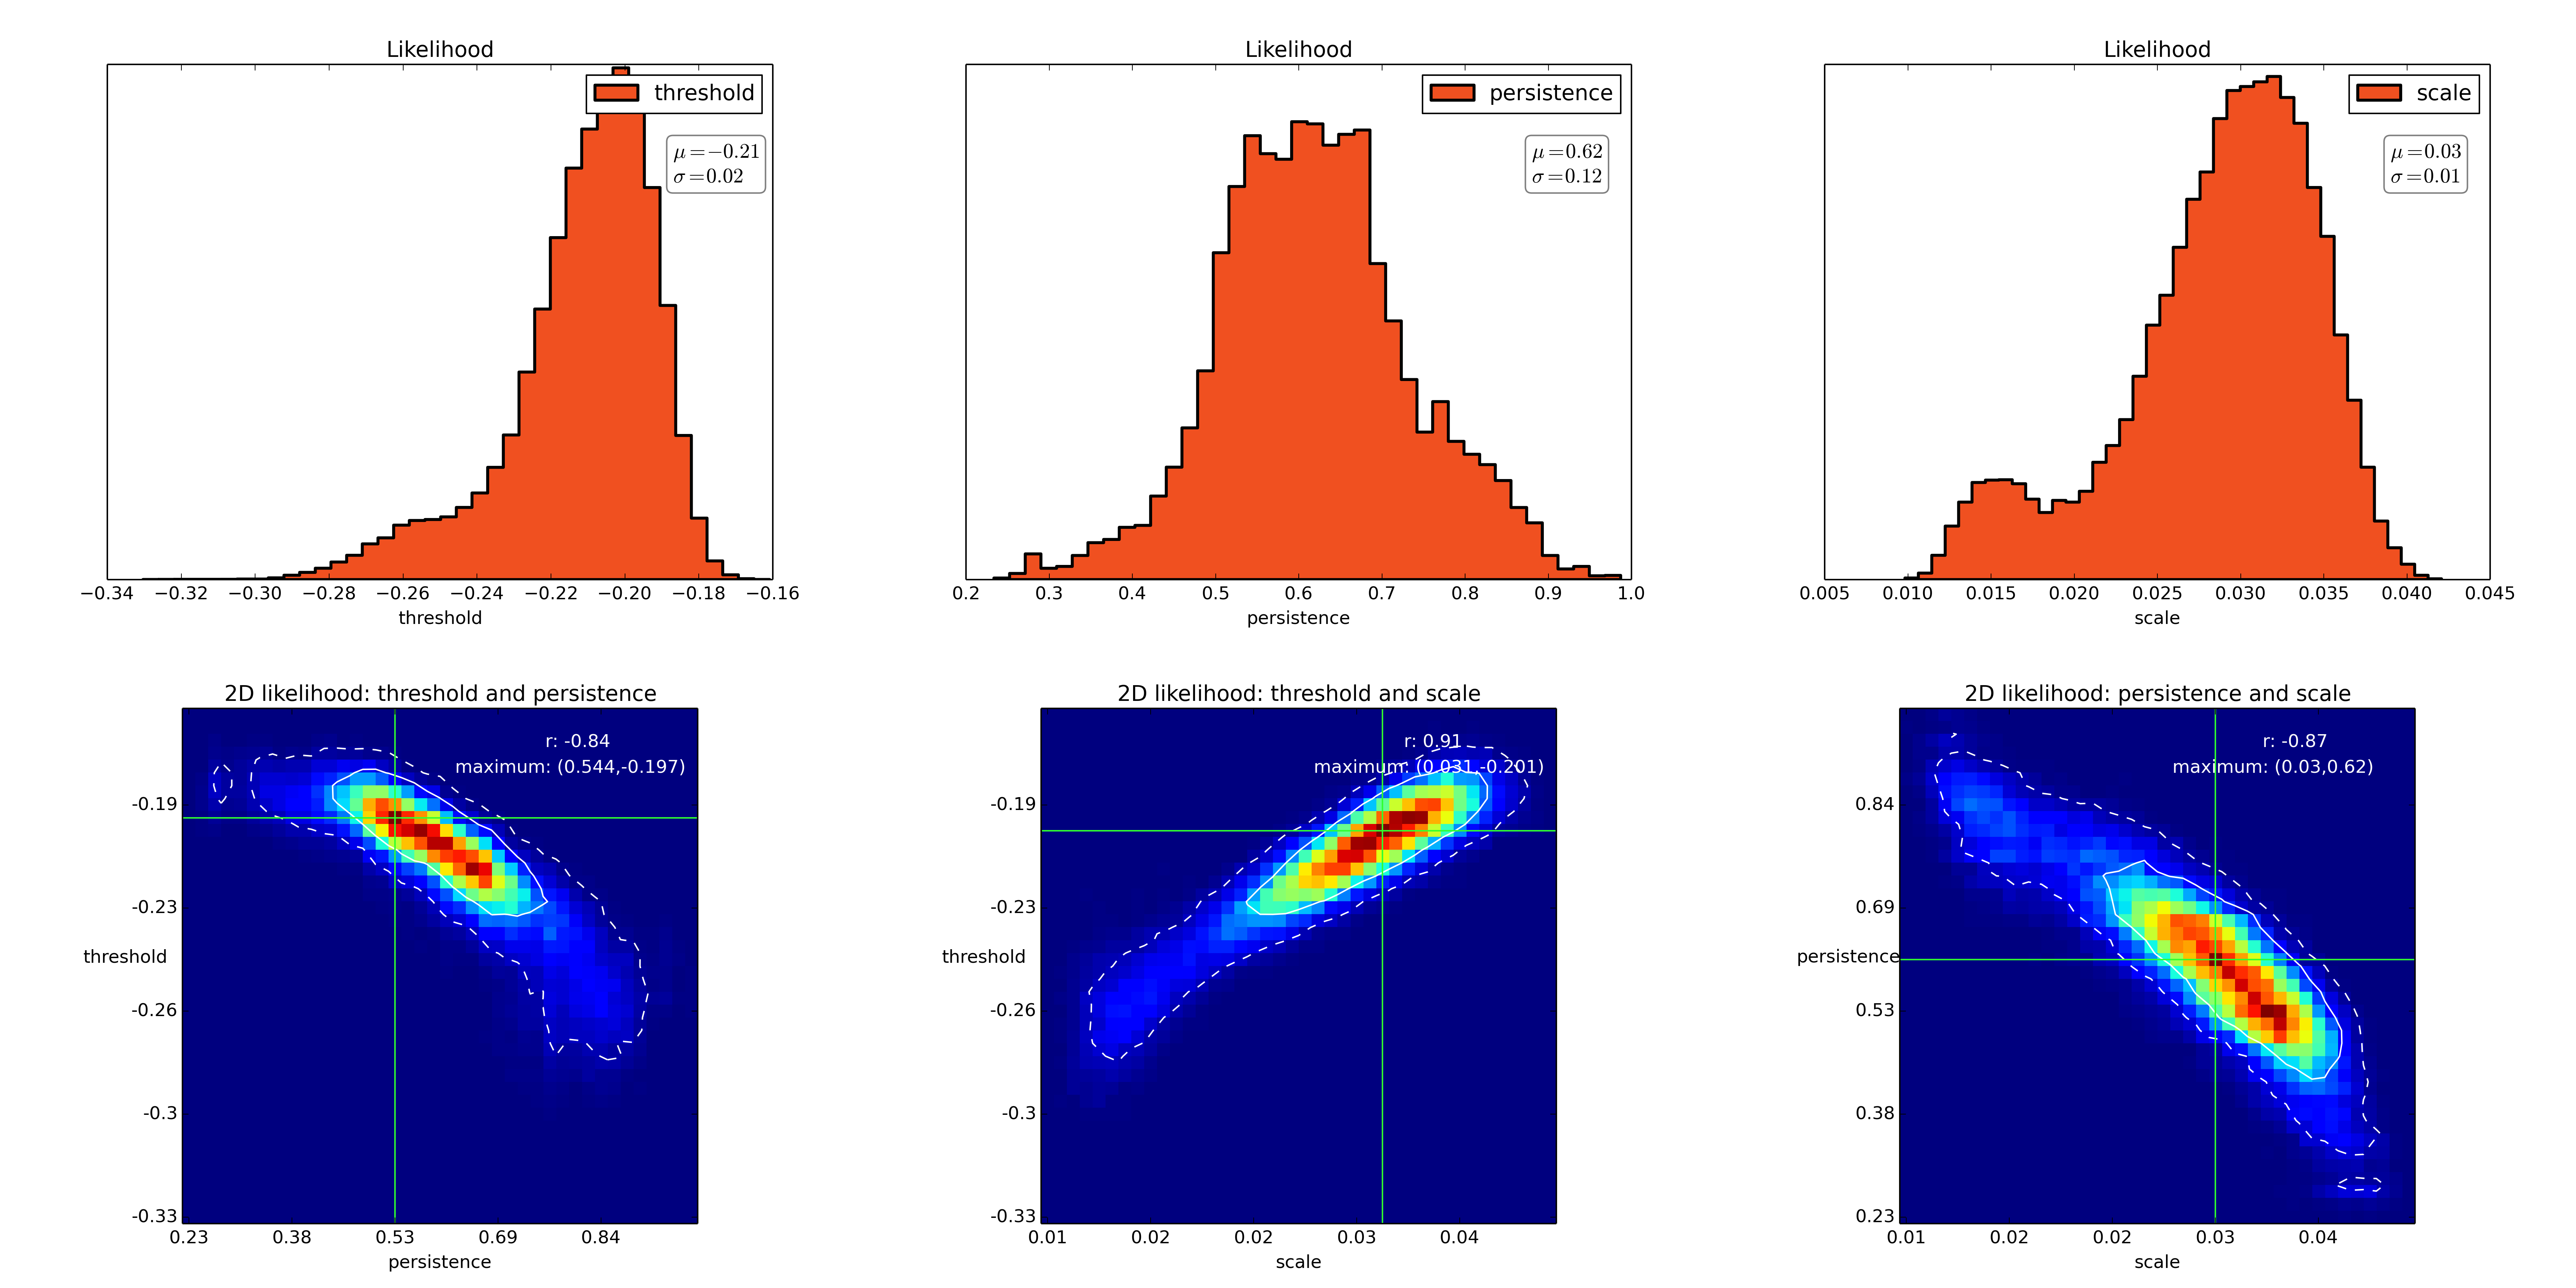
\includegraphics[width=.99\textwidth]{mock_data_results_pts.png}
\caption{Results from the model validation simulation. The upper panel displays the marginalised 1D posteriors for each parameter, while the lower panel depicts the marginalised 2D posteriors. Note that all input parameters were reproduced well within $1\sigma$ (inner contour line).}
\label{fig:mockdataresults_pts}
\end{figure*}





\section{Results}
%\begin{figure}
%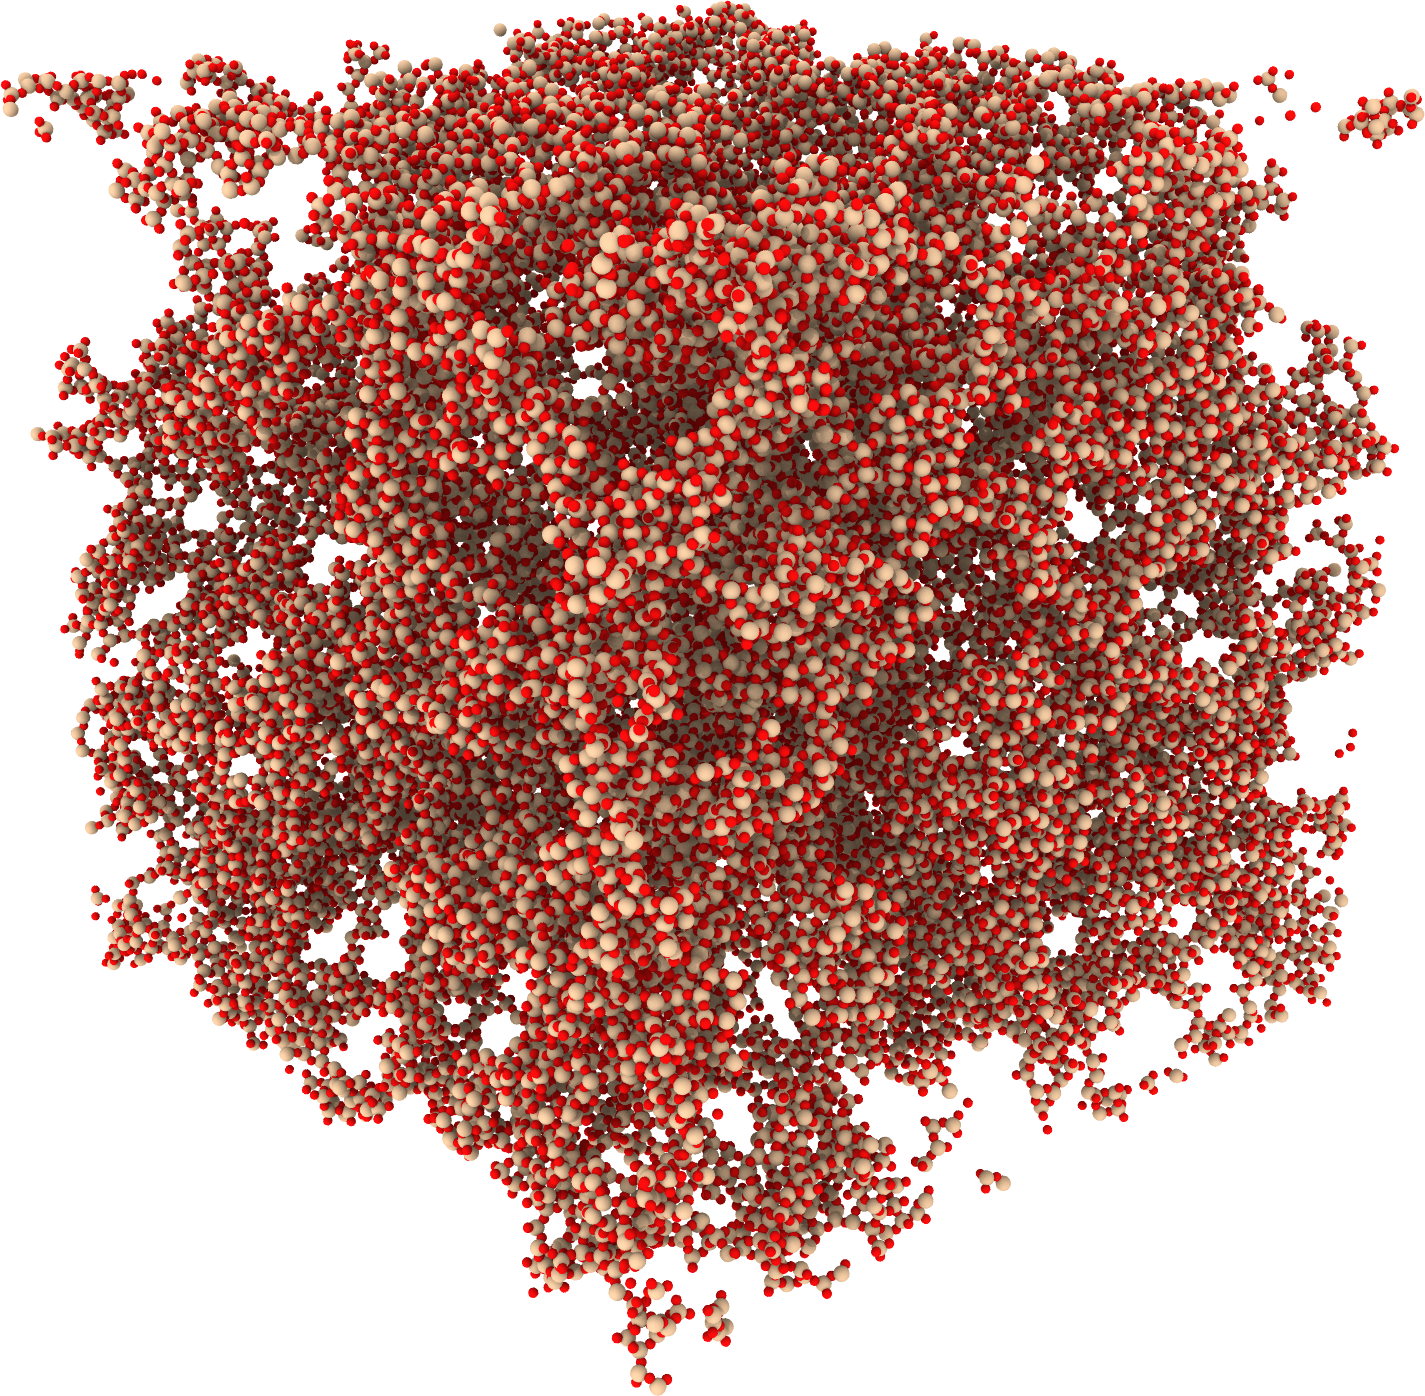
\includegraphics[width=.49\textwidth]{sio_porous.png}
%\caption{Simulated silica created with LAMMPS. The box is $159^3 \AA$, with $100 000$ particles, having been created by cooling an expanding system until quenching was achieved. Note the similarities between the pores here and in figure \ref{fig:mockdata}.}
%\label{fig:si2data}
%\end{figure}
\begin{figure*}
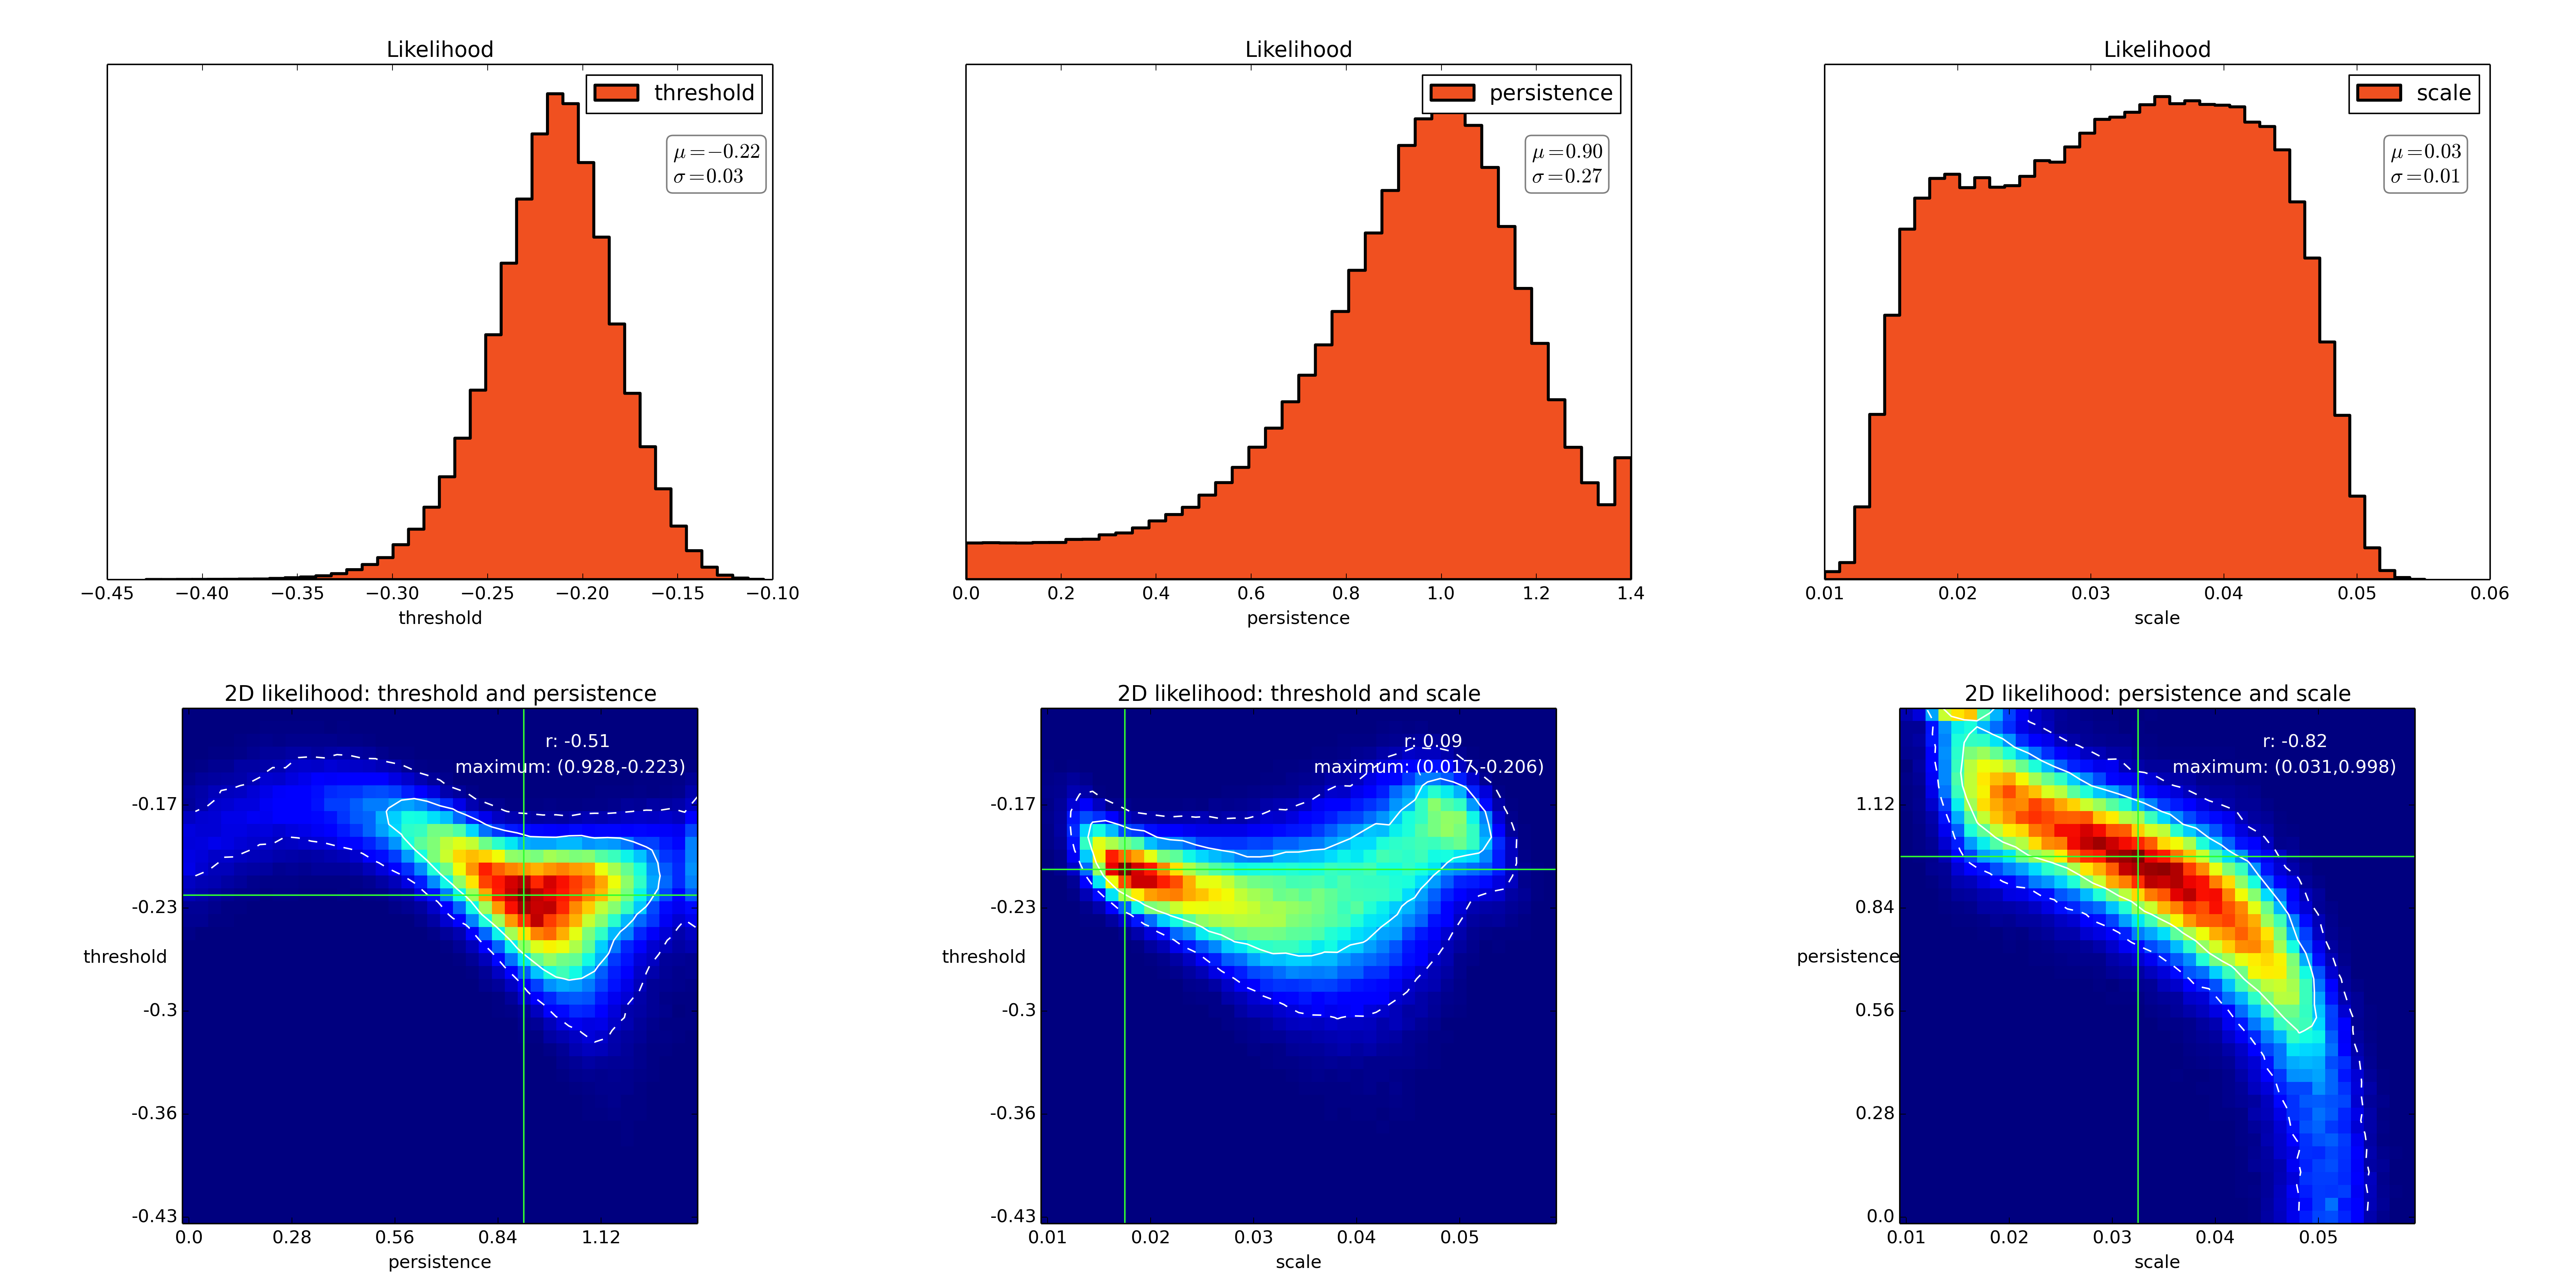
\includegraphics[width=.99\textwidth]{results_porous_full.png}
\caption{Results from the analysis of a simulated $159^3$ \AA $SiO^2$ nanoporous data set. The upper panel displays the marginalised 1D posteriors for each parameter, while the lower panel depicts the marginalised 2D posteriors. Best fit parameters from the maximum 3D likelihood suggest $\tau=-0.2$, $\psi=0.8$ and $\nu=0.3$.}
\label{fig:porous_results1}
\end{figure*}

We now perform a parameter fitting analysis on realistic simulated nanoporous media. Using LAMMPS \cite{plimpton1995fast}, we simulate a $100^3$ \AA box of 100K $SiO^2$ silica particles at an initial temperature of $4500 K$, using the Vashishta-potential. After an initial period, we expand the box to $159^3 \AA$ and start cooling until quenching is achieved at about $300K$. The resulting nanoporous media is depicted in figure \ref{fig:sio2data}, with a porosity of $75\%$.

With the model described in \ref{eq:noisemodel1}, we perform a full likelihood analysis of the data set with the three free parameters $\tau$, $\nu$ and $\psi$ using $g(r)$ as the measure. The resulting marginalised posteriors are depicted in figure \ref{fig:porous_results1}, with best-fit parameters $\tau=-0.2$, $\psi=0.8$ and $\nu=0.3$ is extracted from the full 3D likelihood. We also display the radial pore size distribution $g(r)$ for the input data set, a best-fit parameter data set and a bad-fit data set in figure \ref{fig:gofr1}, to illustrated the sensitivity of $g(r)$ given the model parameters. Note that we are not able to accurately reproduce the structures of the $SiO^2$ $g(r)$ with our current model, but hope that we during future work will be able to produce another model that provides a better fit with this measure. 


\begin{figure}
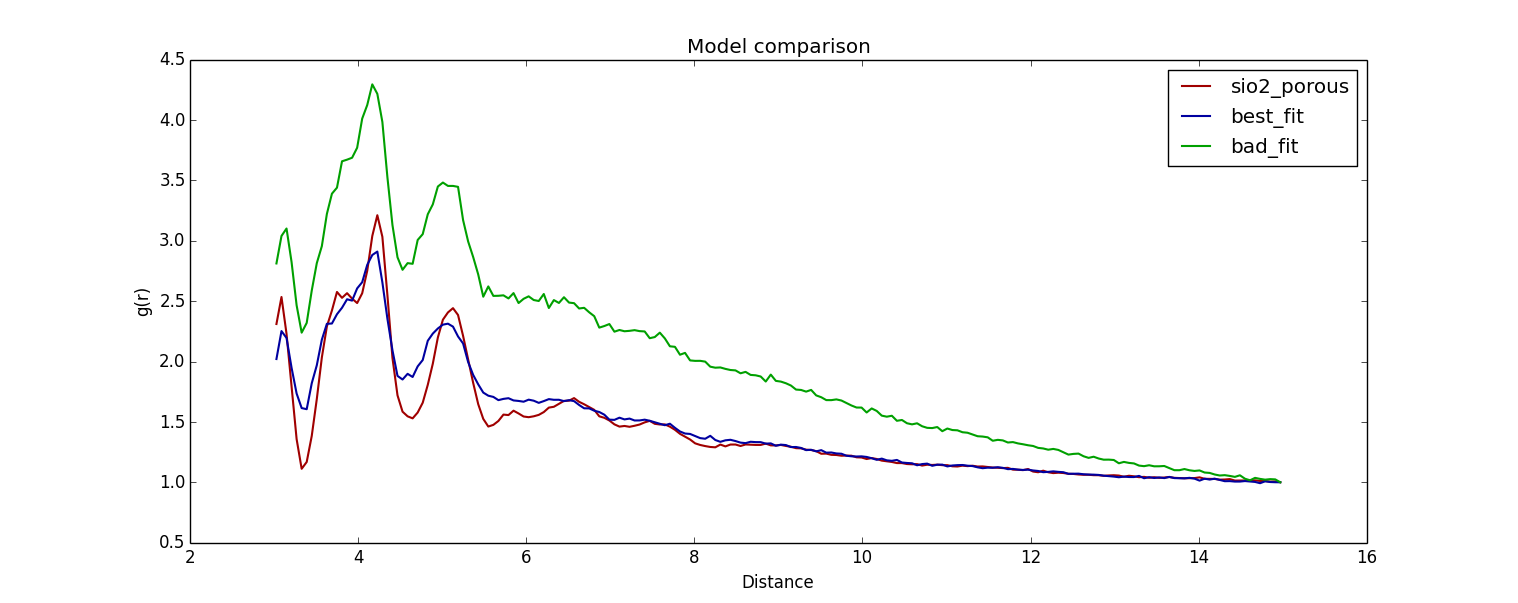
\includegraphics[width=.55\textwidth]{gofr_plot.png}
\caption{The radial pore size distribution $g(r)$ for three data sets: the simulated $SiO^2$ input data set, the best-fit parameter data set and a random low-fit parameter data set. }
\label{fig:gofr1}
\end{figure}
Finally, we depict a comparison of the actual simulated input $SiO^2$ data set together with a representation of the best-fit parameters in figure \ref{fig:porous_vs_model}   
\begin{figure}
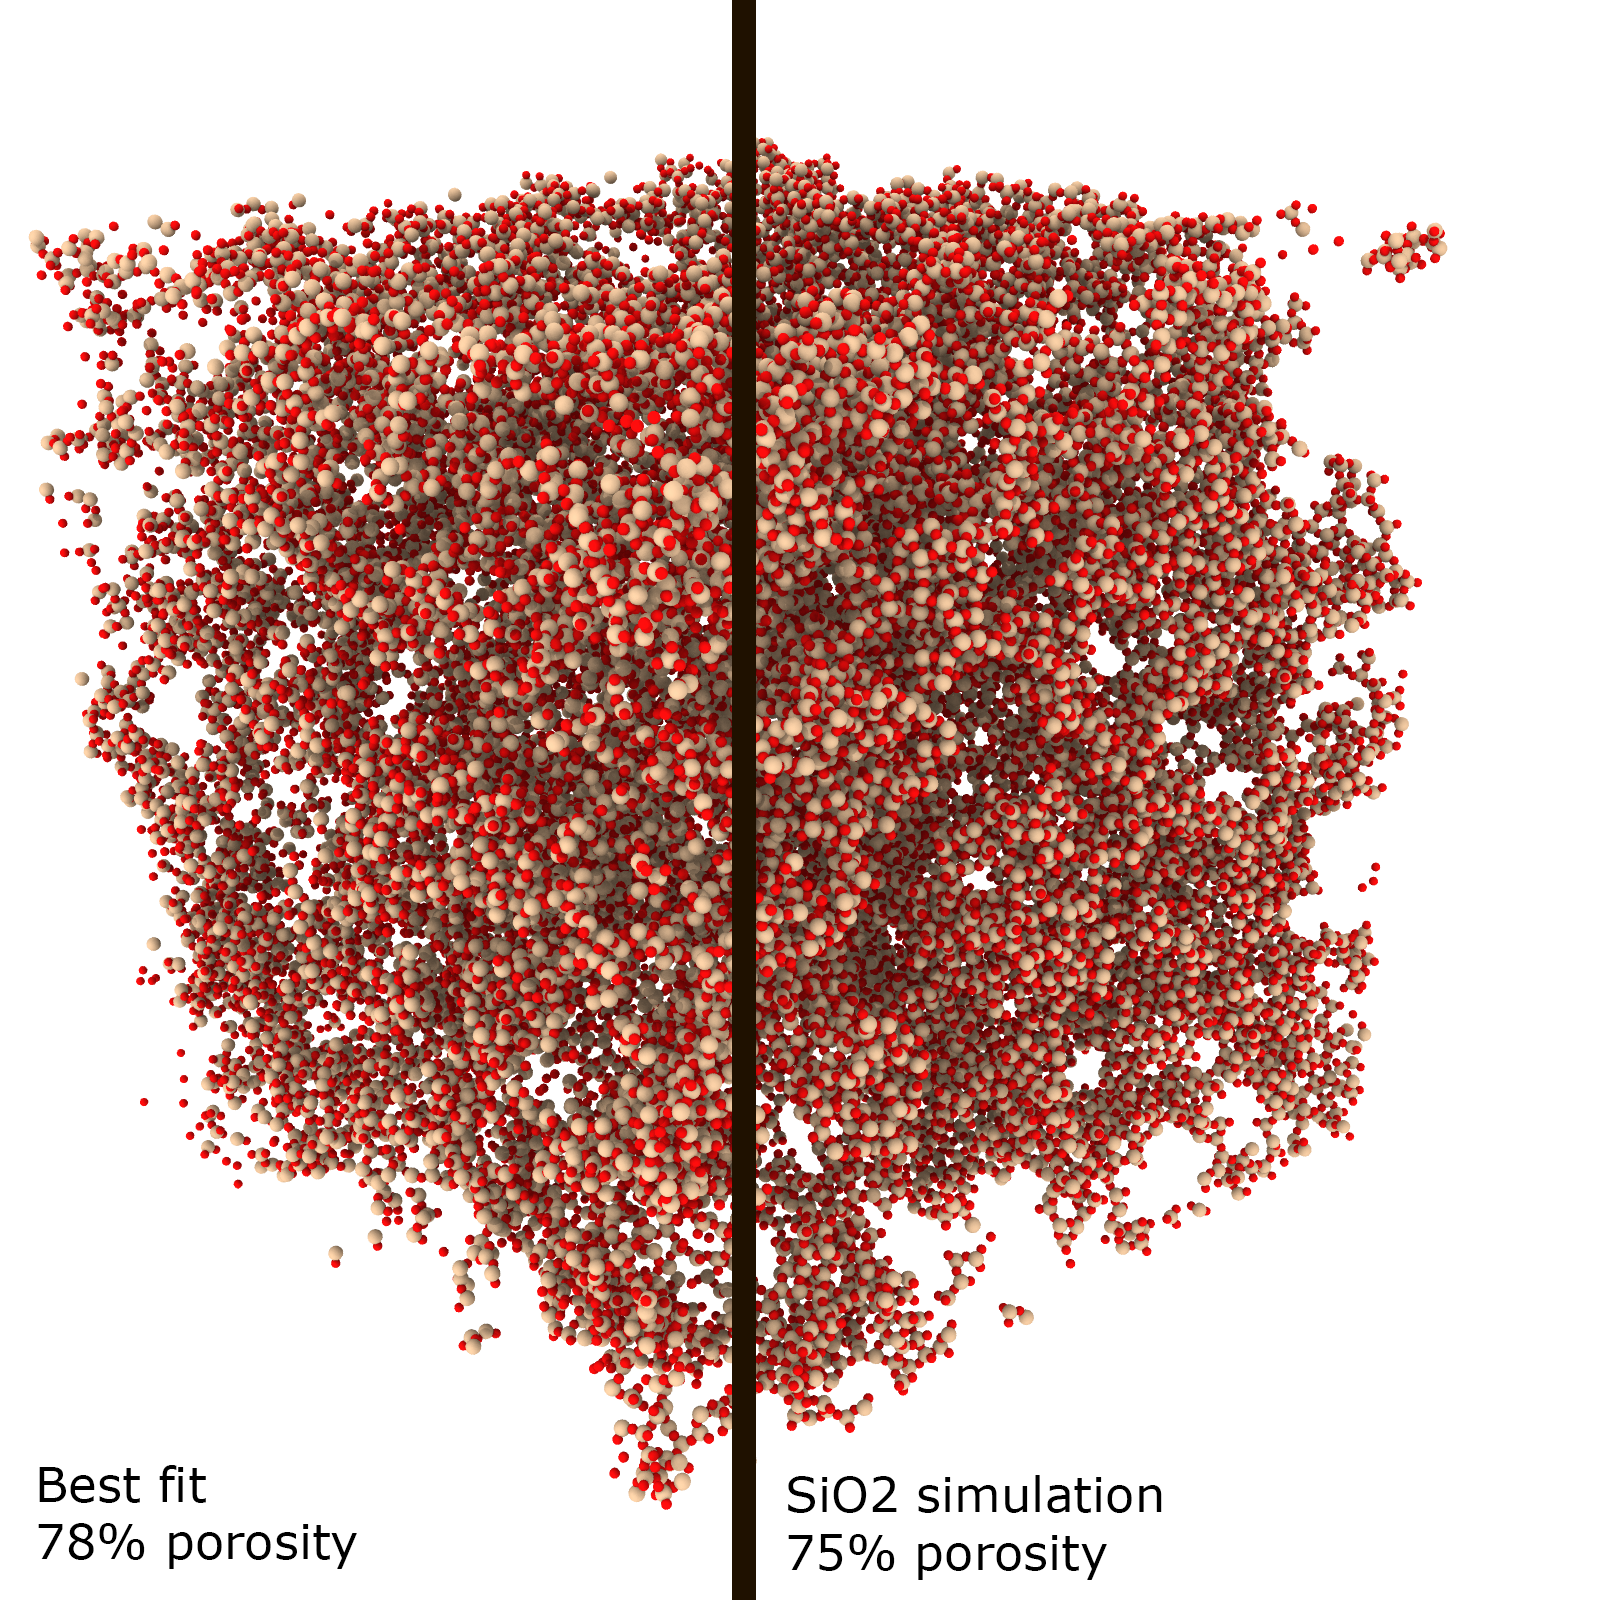
\includegraphics[width=.45\textwidth]{comparison.png}
\caption{Right side: A realisation of the best-fit parameters $\tau=-0.2$, $\psi=0.8$ and $\nu=0.3$. Left side: Simulated $SiO^2$ input data set used for parameter estimation. }
\label{fig:porous_vs_model}
\end{figure}

The porosity of the input $SiO^2$ data set is $75\%$, while the best-fit data set has porosity $77\% \pm 3 \%$, depending on the random seed. In addition, the surface area of the original data set was $\tilde 29 000 \AA^2$, while the best-fit data shows similar values with surface are ranging between $\tilde 28 000 \AA^2$ and $\tilde 30 000 \AA^2$.

\subsection{Some notes on the results}
It is worth to note that since we are chiefly interested in obtaining a set of parameters that reproduces a statistical correct representation of the input data, we are relatively free to choose parameters as desired. In the previous analysis, we selected a best fit threshold value of $\tau=-0.2$, but from the width of the likelihood it is clear that nearby parameters would also be suitable. However, the surface area is strongly correlated with this value, so even slight deviations (e.g. $\Delta \tau = 0.05$) yields a relatively large change in surface area. 

In addition, we do not claim that this model accurately reproduces the pore structure observed in nanoporous simulations, as is evident from the radial pore size distribution shown in figure \ref{fig:gofr1}.



%persistence : 0.875111019125
%scale : 0.036638
%threshold : -0.236784875   78% porosity

% bad fit : scale 0.1, p = 1, threshold = -0.3


\section{Conclusion}
In this paper, we have proposed a novel method for generating a simple kind of nanoporous media using procedural methods, namely Simplex noise. We have developed tools for creating such porous materials, and also estimating model parameters given data. We have shown that it is possible through a full likelihood analysis to reproduce the input parameters of a simulated model. In addition, we performed an analysis on a simulated $159^3 \AA$ data set of $SiO^2$, and explain that while porosity and surface area corresponds well between the model and data, the radial pore size distribution $g(r)$ show that the current model does not exactly reproduce correct data. However, we do not claim that the current model should do so yet, since we have chosen the simplest kind of summation with regards to procedural noise modes. 

\subsection{Future work}
In this paper, we have only considered the simplest kind of procedural noise: a simple sum over modes with threshold cut-off $\tau$, scale fall-off persistence $\psi$ and initial scale $\nu$. We have also seen that, even through both porosity and surface area accurately reproduced, there are features in the radial pore size distribution $g(r)$ that are not fully captured with the current model. This is evident from the images of the simulated structure seen in \ref{fig:porous_vs_model}, where the connecting nearly one-atom thin walls are difficult to reproduce with the current model. However, as procedural noise exert properties closely related to that of fractals, it is possible to extend the number of parameters and define new models with very different properties. Some examples of these models are depicted in figure \ref{fig:future_models}, where the left- and centre images show a new model with two new parameters (offset and gain), while the rightmost panel shows a simulation where the scale $\nu$ is itself being perturbed by procedural noise, yielding strong circular asymmetric patterns.   

Another immediate application would be to estimate model parameters given actual observations of porous media. This would enable us to estimate new parameters such as instrumental noise, deviations from symmetry (yielding asymmetric properties) and  pureness of samples. In addition, by analysing just a few samples and producing an accurate statistical model, we are able to produce an arbitrary amount of statistically correct samples, free from instrumental noise and artefacts. 

A final key analysis would be to compare properties such as percolation through finite-element simulations of gas/liquid flow through our simulated structures, in addition to exerting shear forces, and comparing with actual simulated data from e.g. LAMMPS. 

\begin{figure*}
\includegraphics[width=1\textwidth]{future_models.png}
\caption{Example of future models. Left panel: A multi-fractal model with thin surfaces and large pores. Centre panel: a multi fractal with cave-like structures. Right panel: A model with strong asymmetric noise. }
\label{fig:future_models}
\end{figure*}


Ut hendrerit cursus libero, in scelerisque tortor sollicitudin accumsan. Nam eleifend velit metus, quis volutpat justo faucibus ut. Cras ut sem in nunc fringilla egestas vitae sit amet justo. Ut vel condimentum tortor. Morbi in massa in ipsum ultrices tincidunt. Duis feugiat dignissim nisi ac ultricies. Quisque eget risus fermentum, condimentum massa ullamcorper, posuere neque. Nam congue consequat mi, vel commodo mi tempus eget.

Nullam ultrices, velit sed venenatis ultrices, risus urna ultricies magna, at pretium lorem nibh et nunc. Suspendisse sed mattis leo. Nulla facilisi. Praesent finibus lobortis leo, ut porttitor massa tincidunt ut. Vivamus quis orci eu sem sodales ornare. Cras sed faucibus velit. Phasellus scelerisque mauris quis lorem dignissim vehicula. Sed tempor ut urna sed bibendum. Donec et nibh pulvinar, commodo magna ac, interdum nibh. Sed laoreet ipsum quis quam lacinia, in dictum erat laoreet. Etiam rhoncus mauris arcu, ac egestas lacus facilisis nec. Pellentesque a orci vitae felis faucibus ultrices sed non massa. In posuere vel ex in elementum. Aenean ac neque a enim gravida tristique eu ac lacus. Ut tincidunt venenatis lectus, et maximus mauris.

Proin ornare nulla id tristique placerat. Integer nec elementum tellus. Cras at tempus lectus. Cras lorem est, ornare id condimentum vitae, scelerisque eu lectus. Aenean libero arcu, consequat vel sagittis eget, sagittis ut neque. Pellentesque habitant morbi tristique senectus et netus et malesuada fames ac turpis egestas. Aenean nec quam sodales, mollis est sit amet, vulputate turpis. Praesent tempus diam eu sem laoreet finibus. Nulla finibus, sapien vel lobortis ultricies, mauris ipsum aliquet urna, quis rutrum sapien dui id ipsum. Quisque sodales ex sapien, ac egestas lacus suscipit et. Suspendisse accumsan rhoncus tristique. Pellentesque ut eros lectus. Praesent viverra sit amet odio nec vulputate. Class aptent taciti sociosqu ad litora torquent per conubia nostra, per inceptos himenaeos. Nulla molestie metus vitae libero vulputate, at interdum enim tempus.
\subsection{Simulated data}



%%%%%%%%%%%%%%%%%%%%%%%%%%%%%%%%%%%%%%%%%%%%%%%%%%%%%%%%%%%%%%
%%%%%%%%%%%%%%%%%%%%%%%%%%%%%%%%%%%%%%%%%%%%%%%%%%%%%%%%%%%%%%
\bibliography{bibliography}

%\begin{thebibliography}{9}

%\bibitem[Groeneboom2014]{groeneboom2014} Groeneboom, N.~E., \& Dahle, H.\ 2014, \apj, 783, 138 

%\end{thebibliography}


\end{document}  